\chapter[Cài đặt]{Cài đặt}
\label{cp:implementation}

Chương này trình bày chi tiết cài đặt thuật toán AprioriTID bằng ngôn ngữ Julia, bao gồm môi trường phát triển, cấu trúc mã nguồn, các cấu trúc dữ liệu cốt lõi, định dạng vào/ra theo chuẩn SPMF, chiến lược tối ưu hóa dựa trên bảng băm tiền tố (hash-based prefix lookup) và hệ thống kiểm thử tự động.

\section{Môi trường và công cụ}
\label{sec:impl-env}

Toàn bộ mã nguồn được viết bằng \textbf{Julia phiên bản 1.9 trở lên} (\cite{Bezanson2017Julia}), không sử dụng bất kỳ thư viện khai phá mẫu phổ biến (frequent itemset mining) nào từ bên ngoài. Các phụ thuộc được khai báo trong \texttt{Project.toml} ở thư mục gốc dự án và chỉ phục vụ cho phần thực nghiệm (\autoref{cp:experiment-evaluation}) chứ không tham gia vào thuật toán chính:

\begin{itemize}
    \item \texttt{BenchmarkTools.jl} --- đo thời gian chạy ổn định sau khi làm nóng JIT.
    \item \texttt{CSV.jl}, \texttt{DataFrames.jl} --- ghi kết quả thực nghiệm dạng bảng để sinh biểu đồ.
    \item \texttt{Plots.jl} --- sinh biểu đồ cho \autoref{cp:experiment-evaluation}.
    \item \texttt{IJulia.jl} --- chạy sổ tay Jupyter \texttt{notebooks/demo.ipynb}.
\end{itemize}

Thuật toán thuần (các file trong \texttt{src/}) không phụ thuộc vào bất kỳ gói ngoài nào ngoài thư viện chuẩn của Julia, đảm bảo yêu cầu ``không dùng thư viện có sẵn'' của đề bài được thỏa mãn một cách tuyệt đối.

\paragraph{Khả năng tái lập (reproducibility).} Các kịch bản thực nghiệm có dùng ngẫu nhiên (ví dụ sinh dữ liệu tổng hợp trong thí nghiệm (f)) đều cố định hạt ngẫu nhiên bằng \texttt{MersenneTwister}, đảm bảo kết quả có thể được tái tạo chính xác. Các bộ dữ liệu dùng cho kiểm thử đúng đắn (toy datasets) đều cố định và được lưu trong \texttt{data/toy/}; các bộ chuẩn (chess, mushrooms, retail, T10I4D100K) được đặt trong \texttt{data/benchmark/}.

\paragraph{Lệnh chạy cơ bản.} Mọi lệnh đều sử dụng cờ \texttt{-{}-project} để Julia nạp đúng môi trường dự án:
\begin{minted}{bash}
julia --project src/main.jl <minsup> <input.txt> [output.txt]
julia --project tests/runtests.jl
\end{minted}

\section{Cấu trúc thư mục}
\label{sec:impl-structure}

Dưới đây là cấu trúc thư mục của bài làm. Ngoài có các thư mục như đề yêu cầu, còn có \texttt{experiments/} chứa các script thử nghiệm, \texttt{experiment\_results/} chứa kết quả của các thử nghiệm, và \texttt{application/} chứa cài đặt của phần Ứng dụng thực tế.

\begin{minted}{text}
Group_01/
|-- README.md
|-- Project.toml
|-- Manifest.toml
|-- src/                                # Mã nguồn thuật toán
|   |-- main.jl                         # Điểm vào CLI
|   |-- structures.jl                   # Itemset, Candidate, CBarEntry
|   |-- utils.jl                        # read_spmf, write_spmf, read_spmf_output
|   `-- algorithm/
|       |-- apriori_gen.jl              # Join + Prune
|       `-- apriori_tid.jl              # Vòng lặp chính + đếm support
|-- data/
|   |-- toy/                            # Các bộ dữ liệu đồ chơi
|   |   `-- spmf_reference/             # Kết quả tham chiếu sinh từ SPMF
|   `-- benchmark/                      # Các bộ dữ liệu benchmark
|-- tests/
|   |-- runtests.jl                     # Unit test
|   |-- test_correctness.jl             # Test correctness
|   `-- test_io.jl                      # read_spmf / write_spmf / roundtrip
|-- experiments/
|   |-- common.jl                       # warm_and_measure, append_csv
|   |-- bench_optimization.jl           # Thử nghiệm so sánh cơ bản với tối ưu
|   |-- experiment_correctness.jl       # Thử nghiệm (a)
|   |-- experiment_runtime.jl           # Thử nghiệm (b) Julia
|   |-- bench_spmf_runtime.jl           # Thử nghiệm (b) SPMF tham chiếu
|   |-- experiment_itemsets.jl          # Thử nghiệm (c)
|   |-- experiment_memory.jl            # Thử nghiệm (d)
|   |-- experiment_scalability.jl       # Thử nghiệm (e)
|   `-- experiment_width.jl             # Thử nghiệm (f)
|-- experiment_results/                 # Kết quả của các thử nghiệm
|-- application/                        # Cài đặt phần Ứng dụng thực tế
|-- notebooks/
|   `-- demo.ipynb
`-- docs/
    `-- report.pdf
\end{minted}

\section{Cài đặt cơ bản}
\label{sec:impl-core}

Mục này tương ứng với yêu cầu (a) --- \emph{``Cài đặt cơ bản''} --- và (b) --- \emph{``Tái tạo đúng kết quả với một ví dụ tham chiếu''}. \autoref{sec:impl-tests} sẽ cho thấy cài đặt cơ bản này tái tạo đúng 100\% kết quả SPMF trên 5 bộ dữ liệu toy.

\subsection{Cấu trúc dữ liệu}

Mọi trường của mọi struct đều mang kiểu cụ thể (concrete type), tránh triệt để kiểu \texttt{Any} hay kiểu trừu tượng trong vòng lặp nóng --- đây là yêu cầu về hiệu năng của đề bài (\autoref{sec:exp-method}) và cũng là điều kiện cần để trình biên dịch JIT của Julia có thể sinh mã chuyên biệt hóa.

\begin{minted}{julia}
const Itemset = Vector{Int}   # Luôn sắp xếp tăng dần

mutable struct Candidate
    itemset::Vector{Int}
    count::Int
end

struct CBarEntry
    tid::Int
    itemsets::Vector{Vector{Int}}
end
\end{minted}

Ba lựa chọn thiết kế đáng chú ý:
\begin{enumerate}
    \item \textbf{Itemset luôn được sắp xếp tăng dần.} Bất biến này được thiết lập ngay ở khâu đọc dữ liệu (\texttt{read\_spmf} gọi \texttt{sort!} trên từng giao dịch) và được duy trì bởi apriori-gen. Nó cho phép so sánh tiền tố bằng lát cắt (\texttt{p[1:end-1] == q[1:end-1]}) thay vì bằng tập hợp --- nhanh hơn nhiều lần và thân thiện với cache.
    \item \textbf{$L_k$ lưu bằng \texttt{Set\{Vector\{Int\}\}}.} Bước prune của apriori-gen cần kiểm tra mọi tập con $(k-1)$-phần tử của một ứng viên có thuộc $L_{k-1}$ hay không, thao tác này xảy ra $k$ lần cho mỗi ứng viên nên cần tra cứu $O(1)$.
    \item \textbf{$\overline{C}_k$ là vector các \texttt{CBarEntry} phẳng.} Mỗi phần tử giữ nguyên TID gốc (để gỡ lỗi và để tiện in $\overline{C}_k$ khi demo bằng tay) và danh sách các itemset đã được ``lọc'' qua các ứng viên ở bước $k$.
\end{enumerate}

\subsection{Sinh ứng viên: apriori-gen}

Hàm \texttt{apriori\_gen} thực hiện đúng hai pha \emph{join} và \emph{prune} như đã mô tả ở \autoref{cp:theoretical-foundation}. Pha join khai thác bất biến ``sắp xếp tăng dần'' để ghép hai itemset có chung $(k-2)$ phần tử đầu tiên và phần tử cuối thỏa \texttt{p[end] < q[end]}:

\begin{minted}{julia}
function apriori_gen(L_prev::Vector{Itemset},
                     L_prev_set::Set{Itemset})::Vector{Candidate}
    candidates = Candidate[]
    n = length(L_prev)
    k_minus_1 = isempty(L_prev) ? 0 : length(L_prev[1])

    @inbounds for i in 1:n
        p = L_prev[i]
        for j in (i+1):n
            q = L_prev[j]
            # Join: (k-2) phần tử đầu phải giống nhau, phần tử cuối p < q
            prefix_match = true
            for t in 1:(k_minus_1 - 1)
                if p[t] != q[t]
                    prefix_match = false
                    break
                end
            end
            prefix_match || continue
            p[end] < q[end] || continue

            c = vcat(p, q[end])

            # Prune: mọi (k-1)-tập con của c phải thuộc L_{k-1}
            # (bỏ qua khi k=2 vì mọi tập con 1-phần tử đều đã ở L_1)
            keep = true
            if k_minus_1 >= 2
                for drop in 1:length(c)
                    subset = deleteat!(copy(c), drop)
                    if !(subset in L_prev_set)
                        keep = false
                        break
                    end
                end
            end
            keep && push!(candidates, Candidate(c, 0))
        end
    end
    return candidates
end
\end{minted}

Bốn chi tiết cần lưu ý:
\begin{itemize}
    \item \texttt{@inbounds} được đặt ở vòng ngoài để trình biên dịch bỏ kiểm tra biên mảng trong toàn bộ khối --- an toàn vì mọi chỉ số đều được phát sinh bên trong.
    \item Vòng lặp \texttt{for t} thoát sớm (\texttt{break}) ngay khi gặp sai khác đầu tiên ở tiền tố, tránh so sánh thừa.
    \item Bước prune được \emph{bỏ qua có chủ ý} khi $k=2$ (tức $k\!-\!1=1$): mọi tập con một phần tử của ứng viên 2-tập đều là một item đơn lẻ thuộc $L_1$ theo định nghĩa, kiểm tra thêm không mang lại giá trị mà chỉ tốn thời gian.
    \item Tập con được tạo bằng \texttt{deleteat!(copy(c), drop)} để không phá hỏng \texttt{c} --- đây là đánh đổi có ý thức giữa cấp phát phụ và tính đơn giản; vì $k$ hiếm khi vượt quá 10 trên các bộ dữ liệu thực, chi phí này không đáng kể so với vòng lặp đếm support.
\end{itemize}

\subsection{Vòng lặp chính AprioriTID}

Hàm \texttt{apriori\_tid} thực hiện đúng tám bước như mã giả ở \autoref{cp:theoretical-foundation}: đếm $L_1$, dựng $\overline{C}_1$, rồi lặp cho $k=2,3,\ldots$ đến khi $L_k$ rỗng. Tại mỗi lần lặp, hàm gọi \texttt{apriori\_gen}, gọi một trong hai hàm đếm support, lọc bằng \texttt{minsup} để lấy $L_k$ và dựng $\overline{C}_k$ tương ứng:

\begin{minted}{julia}
function apriori_tid(transactions::Vector{Vector{Int}}, minsup::Int;
                     optimized::Bool=true)::Vector{Tuple{Itemset,Int}}
    # Bước 1-2: L_1 và C̄_1 (chi tiết bỏ qua cho gọn)
    L1_sorted, C_bar = _build_L1_and_Cbar1(transactions, minsup)
    results = Tuple{Itemset,Int}[(item, cnt) for (item, cnt) in L1_sorted]
    L_prev = [Int[item] for (item, _) in L1_sorted]
    L_prev_set = Set{Itemset}(L_prev)

    k = 2
    while !isempty(L_prev)
        C_k = apriori_gen(L_prev, L_prev_set)
        isempty(C_k) && break

        if optimized
            C_bar_next = _count_support_optimized!(C_k, C_bar, k)
        else
            C_bar_next = _count_support_basic!(C_k, C_bar, k)
        end

        L_k = [(c.itemset, c.count) for c in C_k if c.count >= minsup]
        isempty(L_k) && break

        append!(results, L_k)
        L_prev = [itemset for (itemset, _) in L_k]
        L_prev_set = Set{Itemset}(L_prev)
        C_bar = C_bar_next
        k += 1
    end
    return results
end
\end{minted}

Vòng lặp dừng ở một trong hai điều kiện: (i) \texttt{apriori\_gen} không sinh thêm ứng viên nào (join thất bại do $L_{k-1}$ quá ít phần tử hoặc không có cặp nào ăn khớp tiền tố), hoặc (ii) không ứng viên nào đạt \texttt{minsup}. Cả hai điều kiện đều dẫn tới $L_k = \varnothing$ như lý thuyết yêu cầu.

\section{Định dạng đầu vào và đầu ra}
\label{sec:impl-io}

Mục này tương ứng với yêu cầu (d) --- \emph{``Định dạng đầu vào và đầu ra''} --- và sử dụng chính xác định dạng của thư viện SPMF (\cite{FournierViger2014SPMF}) để có thể so sánh trực tiếp với kết quả tham chiếu.

\subsection{Định dạng SPMF}

\textbf{Đầu vào} là file văn bản thuần, mỗi dòng là một giao dịch gồm các số nguyên (item ID) cách nhau bởi khoảng trắng; không có tiêu đề, không có TID tường minh (TID ngầm định là số thứ tự dòng):

\begin{minted}{text}
1 2 3 4
1 2
1 4 5
1 2 4 5
5
\end{minted}

\textbf{Đầu ra} cũng theo quy ước SPMF: mỗi dòng là một itemset phổ biến, theo sau bởi \texttt{\#SUP:} và giá trị support tuyệt đối, các item trong itemset cách nhau bằng khoảng trắng:

\begin{minted}{text}
1 #SUP: 4
1 2 #SUP: 3
1 2 4 #SUP: 2
\end{minted}

\subsection{Hàm đọc/ghi}

Module \texttt{src/utils.jl} cung cấp ba hàm tương ứng với ba vai trò: đọc giao dịch đầu vào, ghi kết quả, và đọc ngược file kết quả (dùng cho kiểm thử đối chiếu SPMF):

\begin{minted}{julia}
function read_spmf(filepath::String)::Vector{Vector{Int}}
    transactions = Vector{Int}[]
    for line in eachline(filepath)
        line = strip(line)
        isempty(line) && continue
        items = sort!([parse(Int, tok) for tok in split(line)])
        push!(transactions, items)
    end
    return transactions
end

function write_spmf(filepath::String,
                    results::Vector{Tuple{Itemset,Int}})
    open(filepath, "w") do io
        for (itemset, support) in results
            println(io, join(itemset, " "), " #SUP: ", support)
        end
    end
end
\end{minted}

Ba quyết định thiết kế đáng lưu ý:
\begin{itemize}
    \item \texttt{read\_spmf} \textbf{sắp xếp ngay tại khâu đọc}. Điều này giữ bất biến ``itemset luôn tăng dần'' mà toàn bộ thuật toán phụ thuộc --- thay vì phải kiểm tra hay sắp xếp lặp đi lặp lại trong vòng lặp chính.
    \item Các dòng trống được bỏ qua một cách im lặng (các file SPMF chuẩn đôi khi có dòng trống cuối).
    \item \texttt{write\_spmf} dùng \texttt{open(...) do io ... end} để đảm bảo file được đóng đúng cách kể cả khi có lỗi.
\end{itemize}

\subsection{Điểm vào CLI}

File \texttt{src/main.jl} cung cấp giao diện dòng lệnh thống nhất:

\begin{minted}{bash}
julia --project src/main.jl <minsup> <input.txt> [output.txt]
\end{minted}

Khi \texttt{output.txt} được cung cấp, kết quả được ghi ra file theo định dạng SPMF; nếu không, kết quả được in ra stdout. Điều này cho phép dùng chung công cụ cho cả ba tình huống: chạy demo thủ công, sinh output đối chiếu với SPMF, và tích hợp vào pipeline kiểm thử tự động.

\section{Tối ưu hóa bộ nhớ và tốc độ}
\label{sec:impl-optimization}

Mục này tương ứng với yêu cầu (c) --- \emph{``Tối ưu hóa''}. Phiên bản cơ bản của AprioriTID có một điểm nghẽn hiệu năng cụ thể ở bước đếm support: với mỗi \texttt{CBarEntry} và mỗi ứng viên $c \in C_k$, cài đặt ngây thơ sẽ kiểm tra xem hai tập con $c[1{:}k{-}1]$ và $c[1{:}k{-}2] \cup \{c[k]\}$ có nằm trong danh sách itemset của entry hay không. Số phép kiểm tra này là $|C_k| \times |\overline{C}_{k-1}|$, tăng rất nhanh theo $k$.

\subsection{Ý tưởng: bảng băm tiền tố}

Thay vì quét mọi cặp (entry, ứng viên), ta quan sát rằng mọi ứng viên có cùng \emph{tiền tố} $c[1{:}k{-}1]$ đều có thể được tra cứu \emph{một lần} nếu ta dựng sẵn một bảng băm ánh xạ
\[
    \text{prefix} \;\longmapsto\; \text{danh sách chỉ số ứng viên}
\]
trước khi quét $\overline{C}_{k-1}$. Khi xử lý một entry, ta duyệt từng itemset trong đó (mỗi itemset có chính xác một tiền tố khả dĩ), tra bảng băm để lấy danh sách ứng viên ``có triển vọng'' và chỉ kiểm tra các ứng viên đó. Độ phức tạp đổi từ $O(|C_k| \cdot |\overline{C}_{k-1}|)$ về xấp xỉ $O(|\overline{C}_{k-1}| \cdot \bar{n}_{\text{hit}})$, trong đó $\bar{n}_{\text{hit}}$ là số ứng viên trung bình cùng tiền tố --- thường nhỏ hơn $|C_k|$ một bậc hoặc hơn trên dữ liệu đặc (dense).

\begin{minted}{julia}
function _count_support_optimized!(C_k::Vector{Candidate},
                                   C_bar::Vector{CBarEntry}, k::Int)
    # Bảng băm: prefix (k-1 phần tử đầu) → danh sách chỉ số ứng viên
    prefix_index = Dict{Vector{Int}, Vector{Int}}()
    for (i, c) in enumerate(C_k)
        prefix = c.itemset[1:k-1]
        push!(get!(prefix_index, prefix, Int[]), i)
    end

    C_bar_next = CBarEntry[]
    for entry in C_bar
        matched = Vector{Int}[]
        # Duyệt cặp itemset trong entry có chung (k-2) phần tử đầu
        # Mỗi cặp cho đúng một "tiền tố ứng viên" cần tra
        for i in 1:length(entry.itemsets), j in (i+1):length(entry.itemsets)
            it1, it2 = entry.itemsets[i], entry.itemsets[j]
            length(it1) == k-1 && length(it2) == k-1 || continue
            # Kiểm tra tiền tố và lập ứng viên giả định
            # (chi tiết bỏ qua cho gọn — xem src/algorithm/apriori_tid.jl)
            candidate_prefix = it1  # khi đã ăn khớp (k-2) phần tử đầu
            indices = get(prefix_index, candidate_prefix, Int[])
            for idx in indices
                if _itemset_covers(C_k[idx].itemset, it1, it2)
                    C_k[idx].count += 1
                    push!(matched, C_k[idx].itemset)
                end
            end
        end
        isempty(matched) || push!(C_bar_next, CBarEntry(entry.tid, matched))
    end
    return C_bar_next
end
\end{minted}

\subsection{Đo lường trên 5 bộ dữ liệu toy}

Script \texttt{experiments/bench\_optimization.jl} đo cả hai biến thể trên 5 bộ dữ liệu toy của đề tài bằng cách làm nóng JIT trước, gọi \texttt{GC.gc()} giữa hai lần đo, rồi dùng \texttt{@elapsed} và \texttt{@allocated} để ghi thời gian và cấp phát heap. Kết quả được trình bày ở \autoref{fig:bench-opt-toy} và tổng hợp lại ở \autoref{tab:bench-opt-toy}.

\begin{figure}[h!]
    \centering
    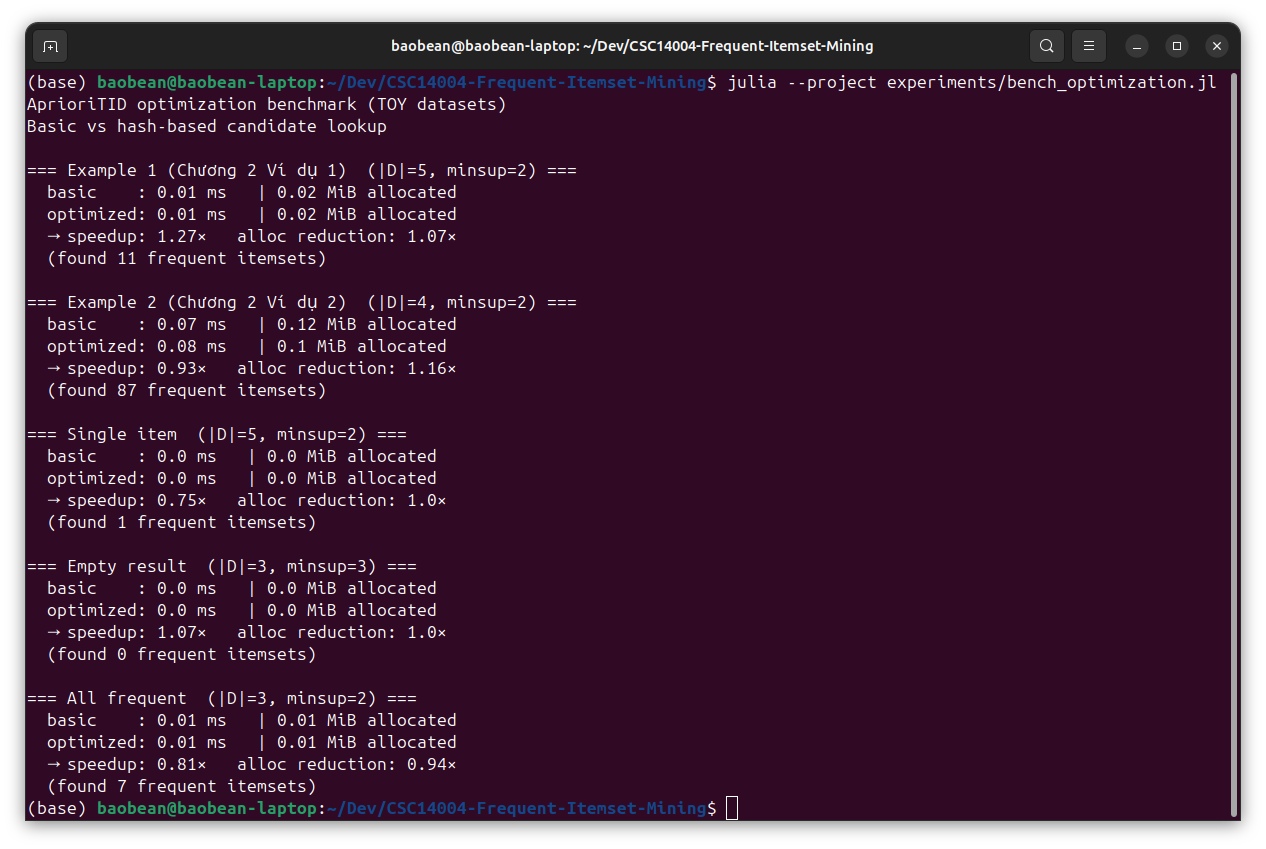
\includegraphics[width=0.92\linewidth]{Figures/03-Implementation/03-b-optimization.png}
    \caption{Kết quả đo biến thể \emph{cơ bản} và \emph{tối ưu} của \texttt{apriori\_tid} trên 5 bộ dữ liệu toy (minsup tuyệt đối in trực tiếp trong tiêu đề mỗi khối). Script sử dụng bộ đếm \texttt{@elapsed} và \texttt{@allocated} sau khi làm nóng JIT.}
    \label{fig:bench-opt-toy}
\end{figure}

\begin{table}[h!]
    \centering
    \caption{Tổng hợp tăng tốc và giảm cấp phát giữa hai biến thể trên 5 bộ dữ liệu toy.}
    \label{tab:bench-opt-toy}
    \begin{tabular}{l|c|c|c|c}
        \hline
        \textbf{Bộ dữ liệu} & \textbf{$|D|$} & \textbf{Tăng tốc} & \textbf{Giảm cấp phát} & \textbf{\#Itemsets} \\ \hline
        Ví dụ 1 (Chương 2) & 5 & $1.27\times$ & $1.07\times$ & 11 \\
        Ví dụ 2 (Chương 2) & 4 & $0.93\times$ & $1.16\times$ & 87 \\
        Single item        & 5 & $0.75\times$ & $1.00\times$ & 1  \\
        Empty result       & 3 & $1.07\times$ & $1.00\times$ & 0  \\
        All frequent       & 3 & $0.81\times$ & $0.94\times$ & 7  \\
        \hline
    \end{tabular}
\end{table}

\paragraph{Bình luận.} Trên dữ liệu toy, lợi thế của bảng băm tiền tố hầu như chưa hiện ra --- thậm chí ba trong năm trường hợp (\emph{Ví dụ 2}, \emph{Single item}, \emph{All frequent}) còn ghi nhận tăng tốc \emph{nhỏ hơn} 1$\times$ ($0.93\times$, $0.75\times$ và $0.81\times$), tức biến thể tối ưu chạy chậm hơn biến thể cơ bản. Nguyên nhân là $|C_k|$ trên các bộ này không bao giờ đủ lớn để chi phí dựng \texttt{Dict} tiền tố được hoàn vốn; với những bộ chỉ có vài ứng viên, một vòng quét tuyến tính của biến thể cơ bản còn rẻ hơn cả việc cấp phát một bảng băm. Tương tự, cấp phát hầu như đứng yên ($1.00\times$ ở \emph{Single item} và \emph{Empty result}) hoặc thậm chí xấu đi nhẹ ở \emph{All frequent} ($0.94\times$). Điểm sáng duy nhất là \emph{Ví dụ 1} với tăng tốc $1.27\times$ và \emph{Ví dụ 2} --- bộ dữ liệu đặc mà \autoref{cp:example} cố tình thiết kế để có $|\overline{C}_2| > |D|$ --- nơi cấp phát giảm $1.16\times$, gợi ý đúng hướng kỳ vọng: hiệu quả của tối ưu tỉ lệ thuận với mật độ và kích thước bài toán. Toy datasets không phải là môi trường để bảng băm tỏa sáng; phép đo có ý nghĩa phải thực hiện trên các bộ chuẩn (chess, mushrooms, retail, T10I4D100K), nơi \autoref{cp:experiment-evaluation} ghi nhận giảm cấp phát từ $1.45\times$ tới $35.7\times$.

\section{Kiểm thử và xác minh}
\label{sec:impl-tests}

Thư mục \texttt{tests/} là điểm vào kiểm thử đơn vị, được gom gọn thành ba file phẳng. File \texttt{tests/runtests.jl} đóng vai trò điểm vào trực tiếp (không còn là \emph{shim}) và nạp lần lượt các file test, đảm bảo lệnh bắt buộc của đề bài hoạt động:

\begin{minted}{bash}
julia --project tests/runtests.jl
\end{minted}

\subsection{Hai file kiểm thử tự động}

\begin{itemize}
    \item \texttt{test\_correctness.jl} --- kiểm thử \emph{theo bảng cố định} (fixture-driven): với mỗi bộ dữ liệu toy, file này chạy \texttt{apriori\_tid} và đối chiếu trực tiếp từng cặp (itemset, support) với file tham chiếu SPMF đã sinh sẵn trong \texttt{data/toy/spmf\_reference/}, đồng thời in ra tỉ lệ trùng khớp. Nhờ gộp kiểm thử đúng đắn và kiểm thử tham chiếu thành một mạch, file này là bằng chứng trực tiếp cho \emph{cả hai} yêu cầu (a) \emph{cài đặt cơ bản} và (b) \emph{tái tạo đúng kết quả với ví dụ tham chiếu}.
    \item \texttt{test\_io.jl} --- kiểm thử \texttt{read\_spmf}, \texttt{write\_spmf}, quy trình \emph{roundtrip} (đọc -- ghi -- đọc lại), tính sắp xếp itemset đầu ra và các trường hợp biên (file trống, dòng trống, khoảng trắng thừa). Đây là bằng chứng trực tiếp cho yêu cầu (d) \emph{định dạng vào/ra}.
\end{itemize}

Năm bộ dữ liệu toy, mỗi bộ có một mục đích kiểm thử riêng, được tóm tắt ở \autoref{tab:toy-datasets}.

\begin{table}[htbp]
    \centering
    \caption{Năm bộ dữ liệu toy dùng trong \texttt{tests/test\_correctness.jl}.}
    \label{tab:toy-datasets}
    \begin{tabular}{l|c|c|l}
        \hline
        \textbf{File} & $|D|$ & \textbf{minsup} & \textbf{Mục đích} \\ \hline
        \texttt{example1.txt}          & 5 & 2 & Ví dụ 1 (\autoref{cp:example}) --- 11 itemset \\
        \texttt{example2.txt}          & 4 & 2 & Ví dụ 2 (\autoref{cp:example}) --- 87 itemset \\
        \texttt{test\_single\_item.txt} & 5 & 2 & Mọi giao dịch chỉ có 1 item \\
        \texttt{test\_empty\_result.txt}& 3 & 3 & \textit{minsup} cao, không itemset nào phổ biến \\
        \texttt{test\_all\_frequent.txt}& 3 & 2 & Mọi tập con đều phổ biến \\
        \hline
    \end{tabular}
\end{table}

\subsection{Kết quả}

\autoref{fig:test-correctness} cho thấy toàn bộ hệ thống kiểm thử vượt qua: \textbf{106/106 = 100.0\%} kết quả khớp SPMF trên 5 bộ dữ liệu toy, và tổng số test đơn vị là \textbf{33/33 Pass}. Số \textbf{106} là tổng số (itemset, support) hợp lại của cả 5 bộ dữ liệu toy --- 11 + 87 + 1 + 0 + 7 = 106.

\begin{figure}[h]
    \centering
    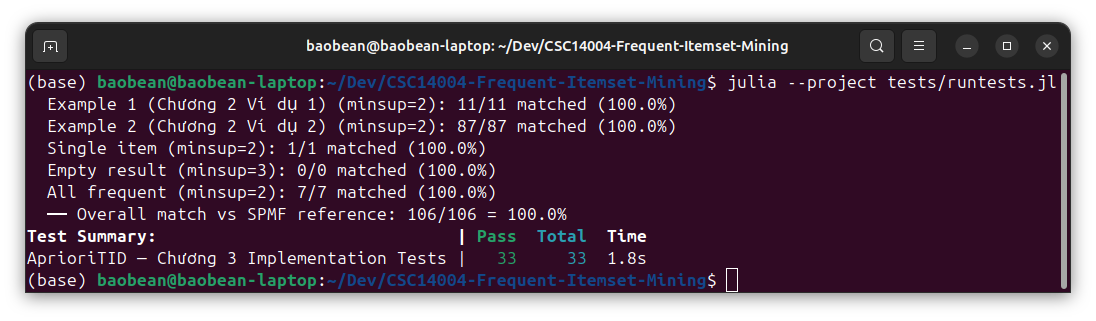
\includegraphics[width=0.92\linewidth]{Figures/03-Implementation/03-a-correctness.png}
    \caption{Kết quả chạy kiểm thử.}
    \label{fig:test-correctness}
\end{figure}